\section{多梯度下降}
\label{sec:moo-mgda}

第~\ref{sec:moo-common-descent}节的判别给出了一个方向：梯度凸包中离原点最近的点。这一节把它变成迭代。问题是：怎样在几个目标的梯度之间取折中，才能保证一步之后每个目标都不变差？

由此得到的方法称为\term{多梯度下降算法}（multiple-gradient descent algorithm，MGDA）。它不需要事先给定偏好，权重是每一步按当前的几何现算的，这一点和固定加权和不同。

\subsection{最小范数组合}
\label{sec:moo-min-norm}

\paragraph{主要思想}
最简单的想法是把各目标的梯度平均一下，然后沿反方向走。看一个具体的数据：
\[
 \bm{g}_1=(10,1),\qquad\bm{g}_2=(-1,1).
\]
平均后得$(4.5,1)$，方向是$\bm{d}=(-4.5,-1)$。检查第二个目标的方向导数：
\[
 \langle\bm{g}_2,\bm{d}\rangle=4.5-1=3.5>0.
\]
$f_2$反而上升。梯度长度悬殊时，长的那个梯度支配了平均，短的那个目标被牺牲了。

\begin{BookInlineFigure}
  \centering
  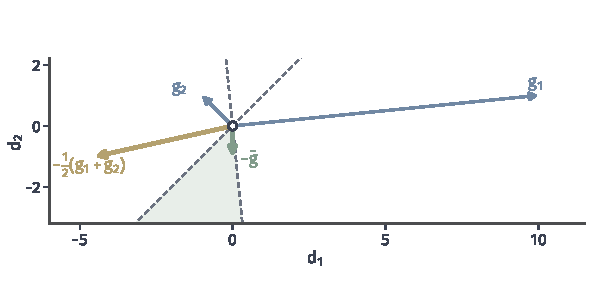
\includegraphics[width=100mm]{figures/05-optimization/07-multiple-criteria-and-nested-optimization/matplotlib/moo-average-vs-minnorm/figure.pdf}
  \caption{平均方向与最小范数方向，$\bm{g}_1=(10,1)$，$\bm{g}_2=(-1,1)$。两条灰色虚线分别垂直于两个梯度，浅绿楔形是共同下降方向。黄色箭头是平均梯度的反方向，落在楔形外；绿色箭头是$-\bar{\bm{g}}=(0,-1)$，落在楔形内。}
  \label{fig:moo-average-vs-minnorm}
\end{BookInlineFigure}

要保证每个目标都下降，应当转而问：在所有梯度的加权平均中，哪一个最短？记
\begin{equation}
 \bm{\theta}^\star\in\argmin_{\bm{\theta}\in\Delta_m}\ \frac12\Bigl\lVert\sum_{i=1}^m\theta_i\bm{g}_i\Bigr\rVert_2^2,
 \qquad
 \bar{\bm{g}}=\sum_{i=1}^m\theta_i^\star\bm{g}_i,
 \label{eq:moo-min-norm}
\end{equation}
并取方向$\bm{d}=-\bar{\bm{g}}$。式~\eqref{eq:moo-min-norm}的权重子问题在单纯形上最小化一个凸二次函数。$\bar{\bm{g}}$是原点在凸包上的投影，所以唯一，而$\bm{\theta}^\star$不一定唯一。

在上面的数据上，后面的式~\eqref{eq:moo-theta-two}给出$\theta_1^\star=1/11$，于是$\bar{\bm{g}}=(0,1)$，方向$(0,-1)$落在共同下降的楔形内，见图~\ref{fig:moo-average-vs-minnorm}。两个方向导数都等于$-1$。

\begin{lemma}[最小范数组合的下降性质]
\label{lem:moo-min-norm}
对式~\eqref{eq:moo-min-norm}定义的$\bar{\bm{g}}$，
\begin{equation}
 \langle\bm{g}_i,-\bar{\bm{g}}\rangle\leq-\lVert\bar{\bm{g}}\rVert_2^2\quad\text{对所有}\ i=1,\ldots,m.
 \label{eq:moo-min-norm-descent}
\end{equation}
并且$\bar{\bm{g}}=\bm{0}$当且仅当$\bm{x}$是无约束的Pareto驻定点。
\end{lemma}

\begin{proof}
不等式已在引理~\ref{lem:moo-gordan}的证明中得到，投影性质给出
\[
 \langle\bm{g}_i,\bar{\bm{g}}\rangle\geq\lVert\bar{\bm{g}}\rVert_2^2,
\]
这对$\bar{\bm{g}}=\bm{0}$也成立。第二句是Pareto驻定的定义：$\bm{0}$在凸包中，当且仅当它到凸包的最短距离为零。
\end{proof}

式~\eqref{eq:moo-min-norm-descent}是整个方法的关键：只要$\bar{\bm{g}}\neq\bm{0}$，每个目标的方向导数都不大于$-\lVert\bar{\bm{g}}\rVert_2^2$，都确实在下降，而且下降速度有统一的下界。

\paragraph{两个目标的闭式解}
$m=2$时，令$\bm{\theta}=(\theta,1-\theta)$，$\bm{g}_1\neq\bm{g}_2$。子问题是一元二次函数：
\[
 \phi(\theta)=\lVert\theta\bm{g}_1+(1-\theta)\bm{g}_2\rVert_2^2=\lVert\bm{g}_2+\theta(\bm{g}_1-\bm{g}_2)\rVert_2^2.
\]
求导令其为零，得到无约束的最小点$\langle\bm{g}_2,\bm{g}_2-\bm{g}_1\rangle/\lVert\bm{g}_1-\bm{g}_2\rVert_2^2$。把它截断到$[0,1]$，由于$\phi$是凸的一元二次函数，截断后仍是区间上的最小点：
\begin{equation}
 \theta^\star=\min\Bigl\{1,\ \max\Bigl\{0,\ \frac{\langle\bm{g}_2,\bm{g}_2-\bm{g}_1\rangle}{\lVert\bm{g}_1-\bm{g}_2\rVert_2^2}\Bigr\}\Bigr\}.
 \label{eq:moo-theta-two}
\end{equation}
若$\bm{g}_1=\bm{g}_2$，任取$\theta$都得到同一个$\bar{\bm{g}}$。

图~\ref{fig:moo-min-norm}是三种情形。(a)垂足落在线段内部，$0<\theta^\star<1$，此时式~\eqref{eq:moo-min-norm-descent}对两个目标都取等号，两个目标下降速度相同。(b)垂足落在线段之外，截断后$\bar{\bm{g}}$就是较短的梯度，方向只对那一个目标是最陡的，另一个目标下降得更快。(c)原点在线段上，$\bar{\bm{g}}=\bm{0}$，停止。

\begin{BookInlineFigure}
  \centering
  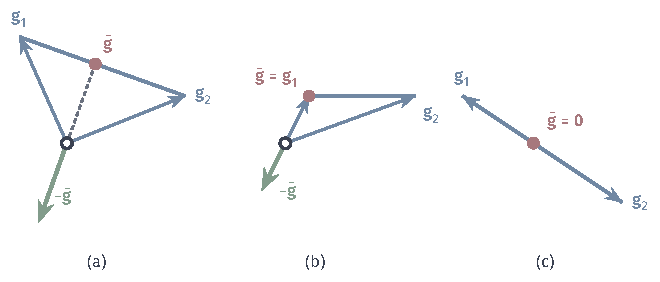
\includegraphics[width=111.8mm]{figures/05-optimization/07-multiple-criteria-and-nested-optimization/tikz/moo-min-norm/figure.pdf}
  \caption{两个梯度的最小范数组合。蓝色线段是凸包，红点是$\bar{\bm{g}}$，绿色箭头是$-\bar{\bm{g}}$，空心点是原点。(a)垂足在线段内部。(b)垂足在线段外，截断到较短的梯度$\bm{g}_1$。(c)原点在线段上，点是Pareto驻定的，没有更新方向。}
  \label{fig:moo-min-norm}
\end{BookInlineFigure}

\paragraph{方向的最优性}
最小范数这个构造还可以从另一面看：它正好是一个“保最差目标”的方向问题的解。假设只看一阶模型，希望下降最少的目标也尽量下降，同时用$\frac12\lVert\bm{d}\rVert_2^2$防止步子过大。

\begin{theorem}[最坏目标的最陡方向]
\label{thm:moo-steepest}
问题
\begin{equation}
 \min_{\bm{d}\in\mathbb{R}^n}\ \max_{1\leq i\leq m}\langle\bm{g}_i,\bm{d}\rangle+\frac12\lVert\bm{d}\rVert_2^2
 \label{eq:moo-steepest}
\end{equation}
的唯一解是$\bm{d}=-\bar{\bm{g}}$，最优值是$-\frac12\lVert\bar{\bm{g}}\rVert_2^2$。
\end{theorem}

\begin{proof}
目标是凸函数加强凸函数，解唯一。对任意$\bm{d}$，最大值不小于凸组合，所以
\[
 \max_i\langle\bm{g}_i,\bm{d}\rangle+\tfrac12\lVert\bm{d}\rVert_2^2
 \geq\langle\bar{\bm{g}},\bm{d}\rangle+\tfrac12\lVert\bm{d}\rVert_2^2.
\]
右端关于$\bm{d}$的最小值在$\bm{d}=-\bar{\bm{g}}$取到，所以
\[
 \max_i\langle\bm{g}_i,\bm{d}\rangle+\tfrac12\lVert\bm{d}\rVert_2^2
 \geq-\tfrac12\lVert\bar{\bm{g}}\rVert_2^2.
\]

反过来，取$\bm{d}=-\bar{\bm{g}}$，由式~\eqref{eq:moo-min-norm-descent}，最大值不超过$-\lVert\bar{\bm{g}}\rVert_2^2$，目标不超过$-\frac12\lVert\bar{\bm{g}}\rVert_2^2$。两边合起来取等，$-\bar{\bm{g}}$是解。
\end{proof}

\paragraph{权重的含义}
$\bm{\theta}^\star$看起来也是一组权重，但它与加权和的权重$\bm{w}$职责不同，见表~\ref{tab:moo-weights}。$\bm{w}$是决策者给定的，整个求解过程中不变，表达的是偏好。$\bm{\theta}^\star$是算法每一步根据当前梯度算出来的，表达的是当前的几何。

\begin{BookInlineTable}
  \centering
  \caption{固定加权与多梯度下降中的权重。}
  \label{tab:moo-weights}
  \begin{tabular}{@{}lll@{}}
    \toprule
     & 加权和的$\bm{w}$ & 多梯度下降的$\bm{\theta}^\star$\\
    \midrule
    来源 & 使用者事先给定 & 每步由梯度算出\\
    迭代中 & 固定 & 随$\bm{x}$变化\\
    单个目标 & 可能上升 & 不上升（配合步长）\\
    终点 & 该偏好下的解 & 取决于起点的一个驻定点\\
    \bottomrule
  \end{tabular}
\end{BookInlineTable}

要注意$\bm{\theta}^\star$不是尺度无关的。把上面的$f_1$除以$10$，$\bm{g}_1$变成$(1,0.1)$，由式~\eqref{eq:moo-theta-two}算得$\theta^\star\approx0.603$，$\bar{\bm{g}}\approx(0.206,0.457)$，方向和原来的$(0,1)$不同。所以第~\ref{sec:moo-scale}节的提醒在这里同样适用：梯度长度悬殊的问题，先要说明目标的尺度。

$m>2$时，令$\bm{G}$是$m\times m$矩阵，元素为$\bm{G}_{i,j}=\langle\bm{g}_i,\bm{g}_j\rangle$，子问题就是在单纯形上最小化$\frac12\bm{\theta}^\top\bm{G}\bm{\theta}$。第~\ref{chap:quadratic-conic-programming}章的二次规划方法和第~\ref{chap:feasible-iterations}章的Frank--Wolfe方法都能解它。单纯形的规模只有$m$，主要开销在于计算$m$个梯度和$\bm{G}$的$O(m^2n)$次运算。

\subsection{共同步长}
\label{sec:moo-common-step}

有了方向，还要决定走多远。若沿各自的梯度分别走一步，再把得到的位置取平均，效果等同于沿平均梯度走一步，前面已经看到这可能让某个目标上升。所以这一小节要为所有目标选一个共同的步长，并检查每一个目标的下降。

\paragraph{多目标的充分下降}
把单目标的回溯规则（第~\ref{chap:smooth-foundations}章）推广：一个步长$\alpha>0$只有在所有目标都达到下面的下降量时才被接受，
\begin{equation}
 f_i(\bm{x}-\alpha\bar{\bm{g}})\leq f_i(\bm{x})-c\,\alpha\lVert\bar{\bm{g}}\rVert_2^2\quad\text{对所有}\ i,
 \label{eq:moo-armijo}
\end{equation}
其中$c\in(0,1)$，常取$c=1/2$。回溯时从$\alpha=1$开始，不满足就乘以$\beta\in(0,1)$，这里取$\beta=1/2$。

为什么步长一定找得到？设每个$\nabla f_i$是$L_i$-Lipschitz的，记$L_{\max}=\max_iL_i$。由下降引理（第~\ref{chap:smooth-foundations}章）和式~\eqref{eq:moo-min-norm-descent}，
\[
 f_i(\bm{x}-\alpha\bar{\bm{g}})
 \leq f_i(\bm{x})+\alpha\langle\bm{g}_i,-\bar{\bm{g}}\rangle+\frac{L_i\alpha^2}{2}\lVert\bar{\bm{g}}\rVert_2^2
 \leq f_i(\bm{x})-\alpha\Bigl(1-\frac{L_i\alpha}{2}\Bigr)\lVert\bar{\bm{g}}\rVert_2^2.
\]
所以当$\alpha\leq1/L_{\max}$时，括号不小于$1/2$，式~\eqref{eq:moo-armijo}在$c=1/2$时成立。

从这里也看得出共同步长的代价：步长受曲率最大的那个目标限制，$L_{\max}$很大时所有目标都得小步前进。

\paragraph{计算过程}
下面在一个病态的例子上走三轮。目标的第一项是第~\ref{chap:smooth-foundations}章贯穿使用的二次函数，第二项把点拉向$(4,3)$：
\begin{equation}
 f_1(\bm{x})=\frac12(x_1^2+9x_2^2),\qquad
 f_2(\bm{x})=\frac12\bigl[(x_1-4)^2+(x_2-3)^2\bigr].
 \label{eq:moo-mgda-example}
\end{equation}

\needspace{6\baselineskip}
\paragraph{变量}
\begin{itemize}
 \item 迭代点$\bm{x}^{(t)}\in\mathbb{R}^n$，各目标的值$f_i(\bm{x}^{(t)})$；
 \item 梯度$\bm{g}_i^{(t)}=\nabla f_i(\bm{x}^{(t)})$，$i=1,\ldots,m$；
 \item 组合系数$\bm{\theta}^{(t)}\in\Delta_m$，组合梯度$\bar{\bm{g}}^{(t)}$；
 \item 步长$\alpha^{(t)}$，常数$c$、$\beta$，容差$\epsilon$。
\end{itemize}

\paragraph{初始化}
给定起点$\bm{x}^{(0)}$和容差$\epsilon$。例中取$\bm{x}^{(0)}=(1,1)$，$c=\beta=1/2$，此时目标值为
\[
 \bm{f}(\bm{x}^{(0)})=(5,\ 6.5).
\]

\paragraph{每轮更新}
对$t=0,1,\ldots$重复下列步骤，直到$\lVert\bar{\bm{g}}^{(t)}\rVert_2\leq\epsilon$。

\begin{enumerate}
 \item 计算各目标的梯度。例中第一轮
 \[
  \bm{g}_1^{(0)}=(1,9),\qquad\bm{g}_2^{(0)}=(-3,-2).
 \]

 \item 由式~\eqref{eq:moo-min-norm}求$\bm{\theta}^{(t)}$与$\bar{\bm{g}}^{(t)}$，两个目标时用式~\eqref{eq:moo-theta-two}。例中第一轮
 \[
  \theta^{(0)}=\frac{34}{137}\approx0.2482,\qquad
  \bar{\bm{g}}^{(0)}\approx(-2.0073,\ 0.7299),
 \]
 并且$\lVert\bar{\bm{g}}^{(0)}\rVert_2^2\approx4.5620$。

 \item 回溯求步长：从$\alpha=1$开始，检查式~\eqref{eq:moo-armijo}是否对每一个目标成立。例中$\alpha=1$的试探点是$(3.0073,0.2701)$，$f_1\approx4.8501$，而要求不超过$5-\frac12\times4.5620\approx2.7190$，被拒绝。$\alpha=1/2$的试探点满足两个目标的要求：
 \[
  f_1\approx3.8220\leq3.8595,\qquad f_2\approx4.7892\leq5.3595.
 \]

 \item 沿$-\bar{\bm{g}}^{(t)}$走一步，更新为
 \begin{equation}
  \bm{x}^{(t+1)}=\bm{x}^{(t)}-\alpha^{(t)}\bar{\bm{g}}^{(t)}.
  \label{eq:moo-mgda-update}
 \end{equation}
 例中第一轮
 \[
  \bm{x}^{(1)}\approx(2.0036,\ 0.6350),\qquad
  \bm{f}(\bm{x}^{(1)})\approx(3.8220,\ 4.7892).
 \]
\end{enumerate}

第二轮的梯度是
\[
 \bm{g}_1^{(1)}\approx(2.0036,\ 5.7153),\qquad
 \bm{g}_2^{(1)}\approx(-1.9964,\ -2.3650).
\]
由此算得
\[
 \theta^{(1)}\approx0.3333,\quad
 \bar{\bm{g}}^{(1)}\approx(-0.6631,\ 0.3283),\quad
 \lVert\bar{\bm{g}}^{(1)}\rVert_2^2\approx0.5475.
\]
$\alpha=1$和$\alpha=1/2$都因$f_1$不满足式~\eqref{eq:moo-armijo}被拒绝，$\alpha=1/4$被接受，得到
\[
 \bm{x}^{(2)}\approx(2.1694,\ 0.5530),\qquad
 \bm{f}(\bm{x}^{(2)})\approx(3.7292,\ 4.6695).
\]

第三轮的梯度是
\[
 \bm{g}_1^{(2)}\approx(2.1694,\ 4.9767),\qquad
 \bm{g}_2^{(2)}\approx(-1.8306,\ -2.4470).
\]
算得
\[
 \theta^{(2)}\approx0.3584,\quad
 \bar{\bm{g}}^{(2)}\approx(-0.3969,\ 0.2138),\quad
 \lVert\bar{\bm{g}}^{(2)}\rVert_2^2\approx0.2032.
\]
同样$\alpha=1/4$被接受，
\[
 \bm{x}^{(3)}\approx(2.2687,\ 0.4995),\qquad
 \bm{f}(\bm{x}^{(3)})\approx(3.6962,\ 4.6250).
\]
可以看到，两个目标每一轮都严格下降，$\theta^{(t)}$在逐轮变化。

最终得到$\bm{x}^\star\approx(2.3933,0.4260)$，目标值约为$(3.6808,4.6034)$，$\bar{\bm{g}}$的范数已到舍入误差量级。这一点的$\theta^\star\approx0.4017$，用它作权重，第~\ref{sec:moo-weighted}节的加权和在这一点取到最优。

\begin{BookInlineFigure}
  \centering
  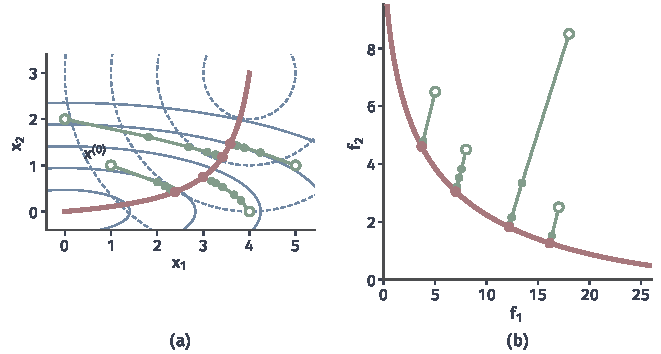
\includegraphics[width=112mm]{figures/05-optimization/07-multiple-criteria-and-nested-optimization/matplotlib/moo-mgda-path/figure.pdf}
  \caption{多梯度下降在例~\eqref{eq:moo-mgda-example}上的路径。(a)决策平面，实线与虚线分别是$f_1,f_2$的等高线，红色曲线是Pareto解集，绿线是四个起点（空心点）的路径，小点是前五步，红点是终点。(b)同一批路径在目标平面上的像，红色曲线是Pareto前沿。不同起点落到前沿的不同位置。}
  \label{fig:moo-mgda-path}
\end{BookInlineFigure}

\paragraph{收敛性}
图~\ref{fig:moo-mgda-path}显示，路径都在目标平面上朝左下方走，最后落到前沿上，不同起点落到不同位置。下面的定理说明能够保证的是什么。

\begin{theorem}[多梯度下降的收敛]
\label{thm:moo-mgda-convergence}
设每个$f_i$有下界$f_i^{\mathrm{low}}$，$\nabla f_i$是$L_i$-Lipschitz的，记$L_{\max}=\max_iL_i$。设迭代满足式~\eqref{eq:moo-armijo}，且$\alpha^{(t)}\geq\alpha_{\min}>0$。则对任意目标$i$和任意$T\geq1$，
\begin{equation}
 \min_{0\leq t<T}\lVert\bar{\bm{g}}^{(t)}\rVert_2^2
 \leq\frac{f_i(\bm{x}^{(0)})-f_i^{\mathrm{low}}}{c\,\alpha_{\min}T}.
 \label{eq:moo-mgda-rate}
\end{equation}
并且序列的每个极限点都是Pareto驻定点。固定步长$\alpha=1/L_{\max}$，$c=1/2$时满足条件，式~\eqref{eq:moo-mgda-rate}的右端为$2L_{\max}(f_i(\bm{x}^{(0)})-f_i^{\mathrm{low}})/T$。
\end{theorem}

\begin{proof}
由式~\eqref{eq:moo-armijo}，对每个$t$，
\[
 f_i(\bm{x}^{(t+1)})\leq f_i(\bm{x}^{(t)})-c\,\alpha_{\min}\lVert\bar{\bm{g}}^{(t)}\rVert_2^2.
\]
对$t=0,\ldots,T-1$求和，利用$f_i(\bm{x}^{(T)})\geq f_i^{\mathrm{low}}$，得到
\[
 c\,\alpha_{\min}\sum_{t=0}^{T-1}\lVert\bar{\bm{g}}^{(t)}\rVert_2^2\leq f_i(\bm{x}^{(0)})-f_i^{\mathrm{low}}.
\]
最小项不超过平均值，即得式~\eqref{eq:moo-mgda-rate}。这一和式也说明$\lVert\bar{\bm{g}}^{(t)}\rVert_2\to0$。

记$\varphi(\bm{x})$为点$\bm{x}$处的$\lVert\bar{\bm{g}}\rVert_2$。对任意$\bm{x},\bm{y}$，设$\bm{\theta}$是$\bm{y}$处的最优系数，
\[
 \varphi(\bm{x})\leq\Bigl\lVert\sum_i\theta_i\nabla f_i(\bm{x})\Bigr\rVert_2
 \leq\varphi(\bm{y})+L_{\max}\lVert\bm{x}-\bm{y}\rVert_2.
\]
交换$\bm{x},\bm{y}$，两式合起来给出
\[
 \lvert\varphi(\bm{x})-\varphi(\bm{y})\rvert\leq L_{\max}\lVert\bm{x}-\bm{y}\rVert_2,
\]
所以$\varphi$连续。沿收敛子列取极限，极限点处$\varphi=0$，由引理~\ref{lem:moo-min-norm}它是Pareto驻定点。

固定步长的情形由式~\eqref{eq:moo-armijo}之后的不等式给出。
\end{proof}

定理的结论是$\lVert\bar{\bm{g}}\rVert_2$趋于零，也就是逼近Pareto驻定。根据第~\ref{sec:moo-common-descent}节，这不等于全局Pareto最优；凸问题中，再加上极限处权重全正，才能推到Pareto最优。回溯时取$\alpha_{\min}=\min\{1,\beta/L_{\max}\}$即可满足定理的条件，因为一旦$\alpha\leq1/L_{\max}$就会被接受。

\paragraph{与固定加权的对比}
图~\ref{fig:moo-mgda-curves}比较了从$(4,0)$出发的两种迭代。这一点的目标值是$(8,4.5)$。固定权重$(1/2,1/2)$的梯度法（黄色）走向该偏好下的解$(2.41,5.64)$，$f_1$降了很多，但$f_2$从$4.5$升到了$5.64$。多梯度下降（绿色）停在$(6.99,3.04)$，两个目标都比起点好。

这两个结果没有谁对谁错。前者忠实地执行了“两项同样重要”的偏好，后者忠实地执行了“不让任何一项变差”的要求。一次运行得到的都只是前沿上的一个点。

\begin{BookInlineFigure}
  \centering
  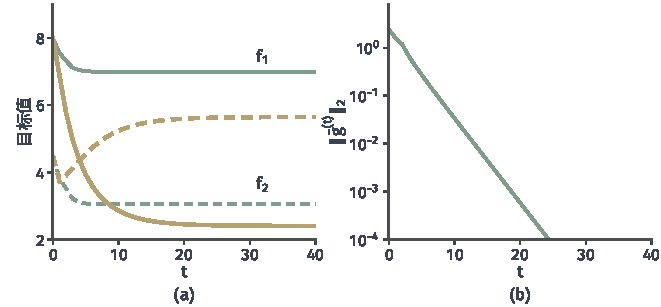
\includegraphics[width=112mm]{figures/05-optimization/07-multiple-criteria-and-nested-optimization/matplotlib/moo-mgda-curves/figure.pdf}
  \caption{从$(4,0)$出发的迭代，例~\eqref{eq:moo-mgda-example}。(a)实线是$f_1$，虚线是$f_2$，绿色是多梯度下降，黄色是固定权重$(1/2,1/2)$、步长$1/L$的梯度法，后者使$f_2$上升。(b)多梯度下降的$\lVert\bar{\bm{g}}^{(t)}\rVert_2$，纵轴为对数。}
  \label{fig:moo-mgda-curves}
\end{BookInlineFigure}

\paragraph{有约束时}
可行集$\bm{C}$是闭凸集时，把式~\eqref{eq:moo-steepest}限制到可行方向上：
\begin{equation}
 \bm{d}^{(t)}\in\argmin_{\bm{x}^{(t)}+\bm{d}\in\bm{C}}\ \max_i\langle\bm{g}_i^{(t)},\bm{d}\rangle+\frac12\lVert\bm{d}\rVert_2^2.
 \label{eq:moo-feasible-direction}
\end{equation}
$\bm{d}=\bm{0}$是可行的，目标值是$0$。由强凸性解唯一，所以$\bm{d}^{(t)}\neq\bm{0}$时最优值严格小于零，$\max_i\langle\bm{g}_i^{(t)},\bm{d}^{(t)}\rangle<0$，$\bm{d}^{(t)}$是共同下降方向。由$\bm{C}$凸，$\bm{x}^{(t)}+\alpha\bm{d}^{(t)}$在$\alpha\in(0,1]$时可行，沿它做共同步长的回溯即可。

反过来，若存在可行点$\bm{x}^{(t)}+\bm{v}$使$\langle\bm{g}_i^{(t)},\bm{v}\rangle<0$对所有$i$成立，取足够小的$\tau>0$，方向$\tau\bm{v}$的目标值就小于零，于是$\bm{d}=\bm{0}$不是解。所以$\bm{d}^{(t)}=\bm{0}$说明从当前点沿可行集内的方向不存在共同下降，这对应第~\ref{sec:moo-feasible-direction}节的驻定条件。$\bm{C}$是多面体时，式~\eqref{eq:moo-feasible-direction}可以写成一个二次规划。

一次多梯度下降通常只给出前沿上的一个点。要得到一组候选，就要进入下一节。
